\chapter{Ship Design}
AAUSHIP1 has been designed by the ASV group during their 6th semester and is extensively designed in a 3D modeling program called RhinoCeros. The plan is to get the ship molded in plastic. As this process is expensive, it's quite important that we agree on the final design of the ship before we send it to the processing company. 

This ship is designed using a tool called Lofting, which takes some lines that runs along the ship, and then generates a surface from these. As none of us have any experience in creating ships - the design is loosely based on what we "think" is a good hull design. 

However, to further strengthen the structure, inlays are made by slicing a box at the edges of the ship hull. These are then to be produced in the machine workshop at the department of electronics. 

To get a better understanding of ship dynamics a rapid prototyping technique have been used, where 3D models of the ship have been printed - and if it didn't live up to our demands (visually deciding if the design was flawed), a revised model was then printed. Using an iterative process - the final design was reached.

\section{Bow thruster}
The ship design includes a bow thruster, which can be used to perform precision maneuvers in tight spaces. This component is not currently included in our control algorithms, because it has little or no effect on the ship when used at speeds above \todo{what speeds?}. It will be controlled by the \ac{LLI} with a direction and a \ac{PWM} signal. 

The electronic design of the bow thruster controller can be found in subsection \ref{subsec:bow thruster controller}: Bow thruster controller.

\section{Ship hull}

The hull of the ship follows a soft-chined displacement design, because in normal operating conditions the static buoyancy will dominate over dynamic. This shape affected less by the currents of the sea, and more by the wind. According to the data series of the British Oceanographic Data Centre\footnote[1]{https://www.bodc.ac.uk/data/online$\_$delivery/nodb/search/} near the shores of Greenland the drift caused by the steady currents is generally higher than the wind with a more randomly distributed blowing direction.

\begin{figure}[hullshape]
	\centering
	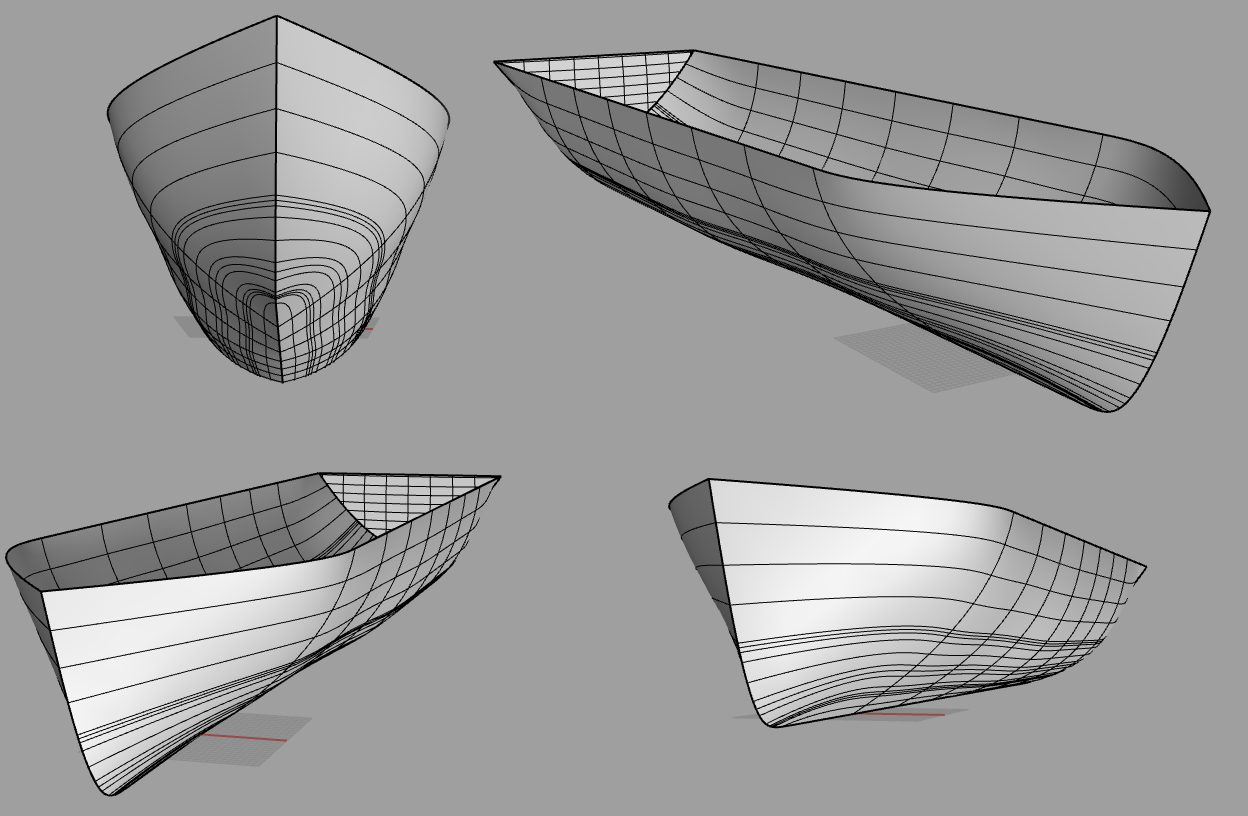
\includegraphics[width=\textwidth]{img/render/rendermontage.png}
	\caption{The shape of the hull}
	\label{fig:vessel-block-overview}
\end{figure}

The ship is outfitted with powerful main engines, so the vessel can perform fast and precise maneuvering without the bow thruster. Though these engines provide a lot of dynamic range, the ship hull was not designed for high speed \ref{jumping}. The problem is caused by the size and power of the propellers. At slower speeds the effect ceases \ref{jumping}.
Mirroring the setup and reversing the rotation movement would solve the pushing problem, but instead the back of the ship is pushed upwards, and air is sucked between the propellers. Instead, an additional vertical fin has been installed above the propellers, which keeps the water from being pushed upwards. As a positive side effect, the water after the hull is significantly less disturbed, thus the drag has been reduced as well. This has a positive effect on the range through the battery life \ref{fin}.

\begin{figure}[jumping]
	\centering
	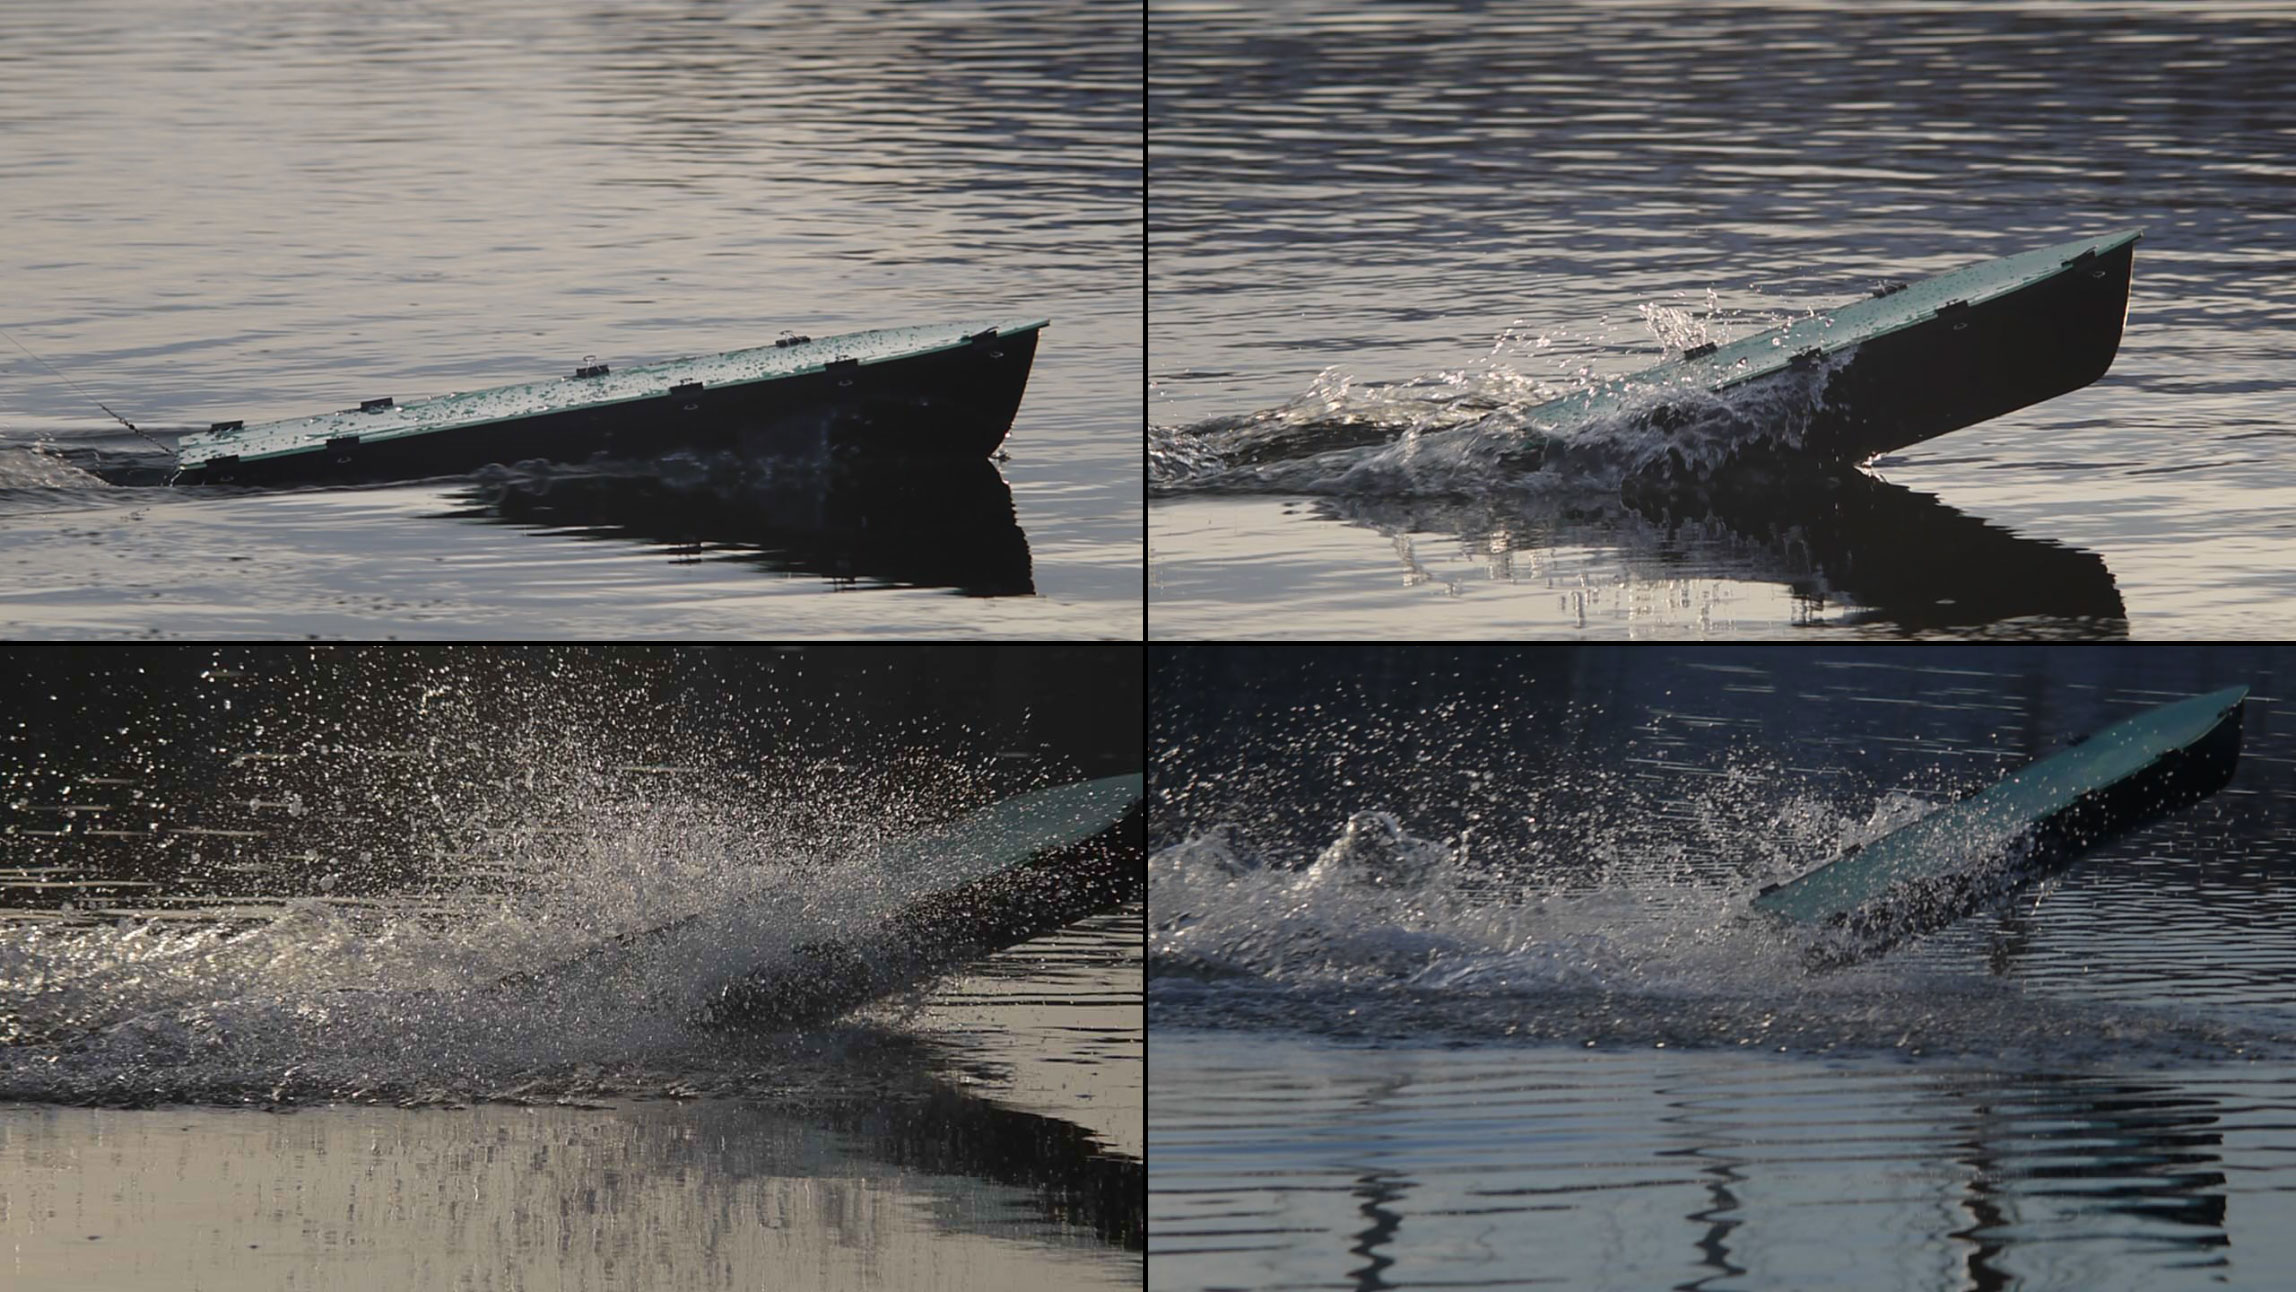
\includegraphics[width=\textwidth]{Pictures/VerticalJumpingTele.jpg}
	\caption{An excessive and unregulated bouncing can be experienced at high speeds.}
	\label{fig:vessel-block-overview}
\end{figure}

\begin{figure}[waterpushup]
	\centering
	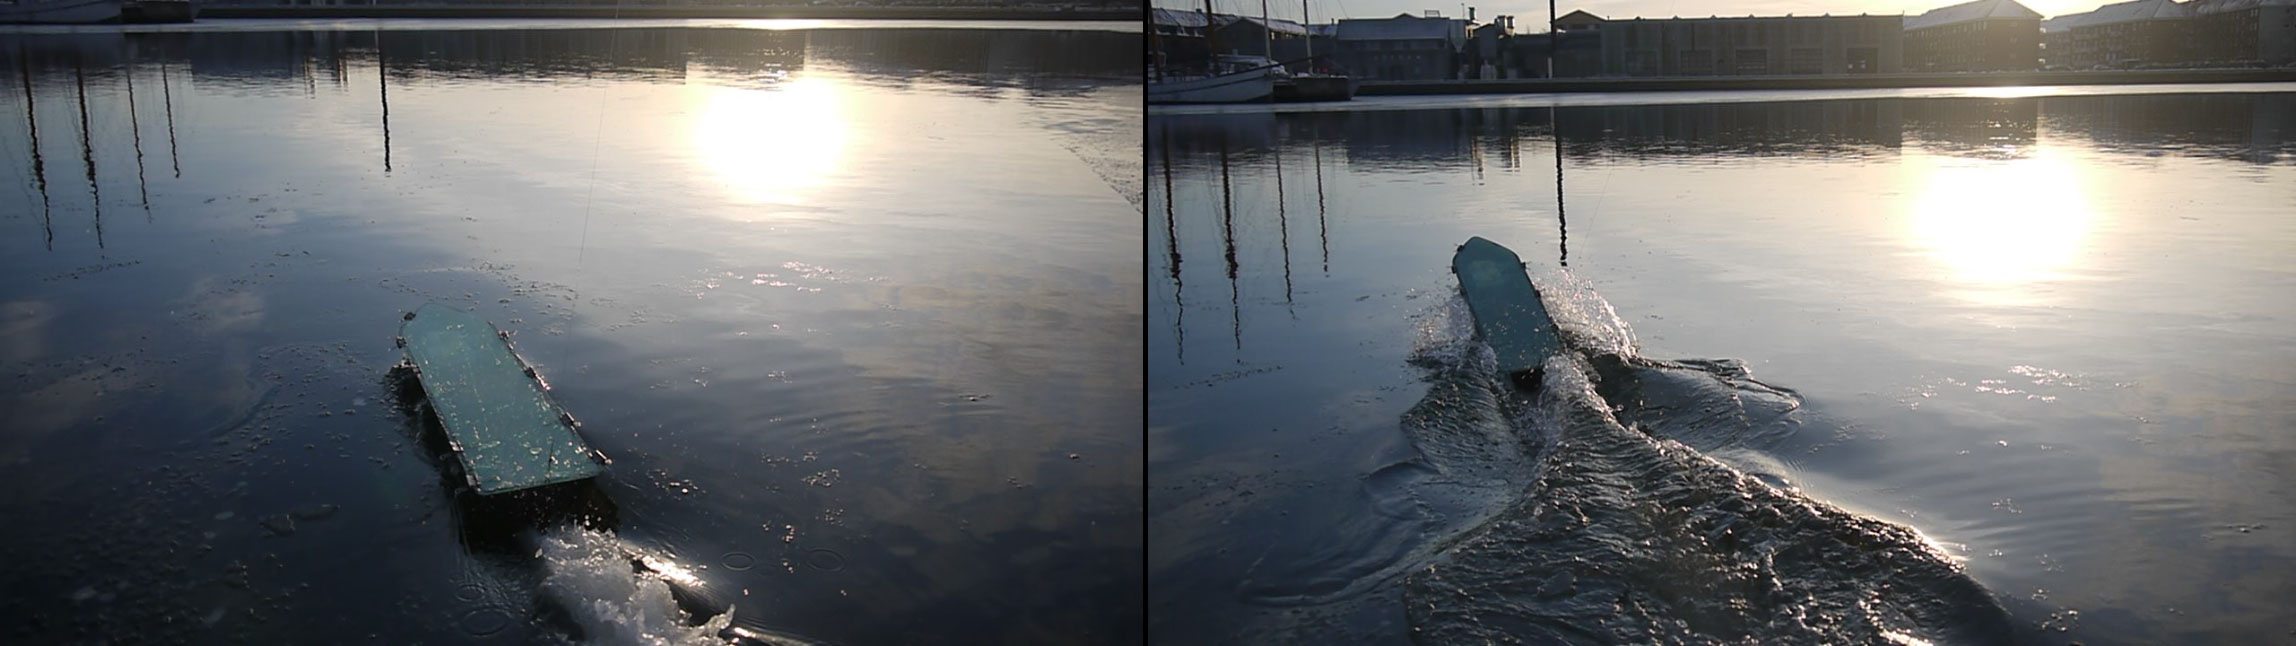
\includegraphics[width=\textwidth]{Pictures/forward.jpg}
	\caption{The power of the two engines force the water upwards between the propellers, therefore pushing the back of the ship down}
	\label{fig:vessel-block-overview}
\end{figure}

\begin{figure}[fin]
	\centering
	\includegraphics[width=\textwidth]{Pictures/Fin.jpg}
	\caption{The rotating propellers with the fin mounted above them. The engine power is set in the normal operation range}
	\label{fig:vessel-block-overview}
\end{figure}

\section{Parts list}
To develop the ship, a wide range of components had to be chosen. There are several things to be taken into consideration when designing a scale ship from scratch. The first component decided upon is the engines. As the ship should be able to cope with rather powerfull streams a powerfull propulsion system had to be chosen. The main propulsion unit consists of 2 Grapuner Brushless 750 14.8 V 1200W engines - which together produces around 3 HP at maximum input. With these powerfull engines we have a large dynamic range, that allows for fast acceleration and a fast maneuvering, as well as navigating in strong currents. 

The propellers are 2 counterrotating Raboesch brass propellers with a radius of 5 cm. 

For power, the ship is fitted with 6 4-celled Lithium-Polymer batteries, each holding up to 3.2 Ah. These will be divided into different sections, 4 serving the main engines, and 2 serving the onboard controls. If the batteries run at full power (draining a maximum of 80 Amps) the ship will be able to sail for 5 minutes, however, a scenario where the engine runs at full power with a brake on the propellers are unlikely.

Measurements show that the engines run at 60/60 (with a 500 max) they drain 2.5As combined, this will give an operation time of 5.1 hours - thus giving quite a big range on the ships. Assuming a 1 m/s velocity kept constantly for 2.5 hours, this gives a range of 9 kilometers forth and 9 kilometers back or being able to measure an area of 1 x 1 km in strips 100 meters apart and still have surplus power.